\begin{center}

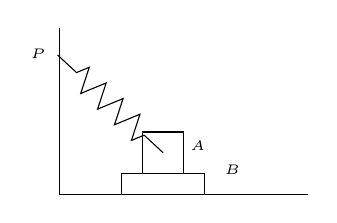
\begin{tikzpicture}[x=0.75pt,y=0.75pt,yscale=-1,xscale=1]
%uncomment if require: \path (0,300); %set diagram left start at 0, and has height of 300

%Straight Lines [id:da7861775888075377] 
\draw    (120,70) -- (120,150) ;
%Straight Lines [id:da5304720563417415] 
\draw    (240,150) -- (120,150) ;
%Shape: Rectangle [id:dp0651080644636306] 
\draw   (150,140) -- (190,140) -- (190,150) -- (150,150) -- cycle ;
%Shape: Rectangle [id:dp9356085279332966] 
\draw   (160,120) -- (180,120) -- (180,140) -- (160,140) -- cycle ;
%Shape: Resistor [id:dp8622106164753849] 
\draw   (119.11,82.88) -- (128.27,91.36) -- (134.41,88.82) -- (130.28,101.44) -- (142.55,96.36) -- (138.42,108.98) -- (150.69,103.9) -- (146.56,116.52) -- (158.83,111.44) -- (154.71,124.06) -- (160.84,121.52) -- (170,130) ;

% Text Node
\draw (105,79) node [anchor=north west][inner sep=0.75pt]  [font=\tiny] [align=left] {$\displaystyle P$};
% Text Node
\draw (182,123) node [anchor=north west][inner sep=0.75pt]  [font=\tiny] [align=left] {$\displaystyle A$};
% Text Node
\draw (198.5,134.5) node [anchor=north west][inner sep=0.75pt]  [font=\tiny] [align=left] {$\displaystyle B$};


\end{tikzpicture}

\end{center}